% Created 2011-02-11 Fr 13:19
\documentclass[bigger]{beamer}
\usepackage[latin1]{inputenc}
\usepackage[T1]{fontenc}
\usepackage{fixltx2e}
\usepackage{graphicx}
\usepackage{longtable}
\usepackage{float}
\usepackage{wrapfig}
\usepackage{soul}
\usepackage{textcomp}
\usepackage{marvosym}
\usepackage{wasysym}
\usepackage{latexsym}
\usepackage{amssymb}
\usepackage{hyperref}
\tolerance=1000
\usepackage{color}
\usepackage{listings}
%%\mode<beamer>{\usetheme{Madrid}}
\usepackage{lucidabr}
\usepackage{marvosym}
\AtBeginSection[]{\begin{frame}<beamer>\frametitle{Topic}\tableofcontents[currentsection]\end{frame}}
\usepackage{cclicenses}
\hypersetup{colorlinks=true, urlcolor=cyan, linkcolor=black}
\providecommand{\alert}[1]{\textbf{#1}}
\begin{document}



\title{Dynamic documents with R and \LaTeX{} as an important part of reproducible research}
\author{Bernd Weiss\\Research Institute for Sociology\\University of Cologne\\Germany\\}
\date{02/11/2011 \vfill \byncsa}
\maketitle

\begin{frame}
\frametitle{Outline}
\setcounter{tocdepth}{3}
\tableofcontents
\end{frame}





\newcommand{\infobox}[1]{
  \vfill\vfill\hrule
  \begin{columns}[t]
    \begin{column}{0.02\textwidth}
      \Info
    \end{column}
    \begin{column}[T]{0.97\textwidth}
      \tiny{#1}
    \end{column}
\end{columns}}

\definecolor{dkgreen}{rgb}{0,0.5,0}
\definecolor{dkred}{rgb}{0.5,0,0}
\definecolor{gray}{rgb}{0.5,0.5,0.5}
\lstset{basicstyle=\ttfamily\bfseries\footnotesize,
morekeywords={virtualinvoke},
%%keywordstyle=\color{blue},
%%ndkeywordstyle=\color{red},
commentstyle=\color{dkred},
%%stringstyle=\color{dkgreen},
numbers=left,
numberstyle=\ttfamily\tiny\color{gray},
stepnumber=1,
numbersep=10pt,
backgroundcolor=\color{white},
tabsize=4,
showspaces=false,
showstringspaces=false,
xleftmargin=.23in
}


\begin{frame}\frametitle{Acknowledgment, license and downloads}
\begin{itemize}
\item This work was supported by a fellowship within the Postdoc-Programme of the German Academic
  Exchange Service (DAAD)(Grant D/10/43517).
\item My presentation was created using Emacs' \href{http://orgmode.org/}{\emph{org-mode}} and
\href{http://orgmode.org/worg/org-contrib/babel/}{\emph{Babel: active code in
Org-mode}}. 
\item Licensed under a Creative Commons
\href{http://creativecommons.org/licenses/by-nc-sa/3.0/de/deed.en}{Attribution-NonCommercial-ShareAlike
3.0 Germany} license.
\item Slides, dataset and R code can be downloaded from my
\href{https://github.com/berndweiss/dynamic_documents_with_r}{github}
page: (see "Downloads" button on the right-hand side).
\end{itemize}
\end{frame}



\section{Preliminary remarks}
\label{sec-1}
\begin{frame}
\frametitle{Outline}
\label{sec-1_1}
\begin{itemize}

\item Present some ideas about reproducible research\\
\label{sec-1_1_1}%
\item My data analysis workflow\\
\label{sec-1_1_2}%
\item \LaTeX in 5 minutes\\
\label{sec-1_1_3}%
\item Sweave: Dynamic documents with R and \LaTeX\\
\label{sec-1_1_4}%
\end{itemize} % ends low level
\end{frame}
\section{Reproducible research}
\label{sec-2}
\begin{frame}
\frametitle{What is reproducible research?}
\label{sec-2_1}


``By reproducible research, we mean research papers with accompanying software tools that allow the
reader to directly reproduce the results and employ the methods that are presented in the research
paper'' (Gentleman/Lang 2004: 1). 
\end{frame}
\begin{frame}
\frametitle{Requirements for the workflow: TREMMP}
\label{sec-2_2}

\small
\begin{itemize}

\item Transparency (e.g., by using dynamic documents, "The source code is real")\\
\label{sec-2_2_1}%
\item Reproducibility (e.g., by using dynamic documents, "The source code is real")\\
\label{sec-2_2_2}%
\item Efficiency (a good workflow saves you time, by automating as much of the process as possible)\\
\label{sec-2_2_3}%
\item Maintainability (standardized script names, good commenting practices, README files)\\
\label{sec-2_2_4}%
\item Modularity (discrete tasks into separate components (e.g. scripts))\\
\label{sec-2_2_5}%
\item Portability (e.g., by using relative (not absolute) pathnames)\\
\label{sec-2_2_6}%
\vfill
\tiny
(Source: David Smith on ``A workflow for R'': \href{http://blog.revolutionanalytics.com/2010/10/a-workflow-for-r.html}{http://blog.revolutionanalytics.com/2010/10/a-workflow-for-r.html})


\end{itemize} % ends low level
\end{frame}
\begin{frame}
\frametitle{Sweave as a tool for creating dynamic documents}
\label{sec-2_3}


``Sweave is a tool that allows the R code used for a complete data analysis to be embedded into
\LaTeX{}, HTML or OpenOffice documents. The purpose is to create dynamic reports, which can be updated
automatically if the data or analysis change. Instead of inserting a prefabricated graph or table
into the report, the master document contains the R code necessary to obtain it. When run through R,
all data analysis output (tables, graphs, etc.) is created on the fly and inserted into a final
document. Data, code and documentation are tightly linked together, which allows for truly
reproducible research'' (Leisch 2010, \href{http://user2010.org/tutorials/Leisch.html}{http://user2010.org/tutorials/Leisch.html}). 

  
\end{frame}
\begin{frame}
\frametitle{Some Sweave examples}
\label{sec-2_4}
\begin{itemize}

\item Dissertation thesis\\
\label{sec-2_4_1}%
\item Medical report with tables and figures\\
\label{sec-2_4_2}%
\end{itemize} % ends low level
\end{frame}
\begin{frame}
\frametitle{The source code is real}
\label{sec-2_5}


``The source code is real. The objects are realizations of the source code. Source for EVERY user
modified object is placed in a particular directory or directories, for later editing and retrieval''
(Rossini et al. 2011:\href{http://ess.r-project.org/Manual/ess.html}{ ESS - Emacs Speaks Statistics - Manual})
\end{frame}
\begin{frame}[fragile]
\frametitle{How my project(s) are organized}
\label{sec-2_6}




\begin{lstlisting}
total 16
-rw-r--r-- 1 1073 Nov  5 08:33 README
drwxr-xr-x 1 4096 Jan 30 10:14 data/
drwxr-xr-x 1    0 Jan 26 12:13 docs/
drwxr-xr-x 1    0 Feb  4 08:11 graphs/
drwxr-xr-x 1    0 Jan 29 16:39 libs/
drwxr-xr-x 1    0 Dec 23 09:34 org/
drwxr-xr-x 1 4096 Feb  4 08:11 reports/
drwxr-xr-x 1 4096 Jan 30 08:03 src/
drwxr-xr-x 1    0 Jan 29 11:44 tests/
\end{lstlisting}
\end{frame}
\section{\LaTeX in 5 minutes}
\label{sec-3}
\begin{frame}
\frametitle{What is \LaTeX}
\label{sec-3_1}
\begin{itemize}

\item \LaTeX{} is a markup language. Another markup language you might know is HTML.\\
\label{sec-3_1_1}%
\item \LaTeX{} provides high-quality typesetting features.\\
\label{sec-3_1_2}%
\item The typical workflow is as follows:
\label{sec-3_1_3}%
\begin{enumerate}
\item Create \LaTeX{} source code file (\texttt{.tex})
\item Compile it via \LaTeX{} or pdf\LaTeX
\item Use a viewer (PDF, DVI or via dvips PS) to view the compiled file
\end{enumerate}

\item In order to run \LaTeX{} on your computer, you will need to install a\\
\label{sec-3_1_4}%
\LaTeX-distribution (e.g., Mik\TeX{} for MS-Windows).  

 

\end{itemize} % ends low level
\end{frame}
\begin{frame}


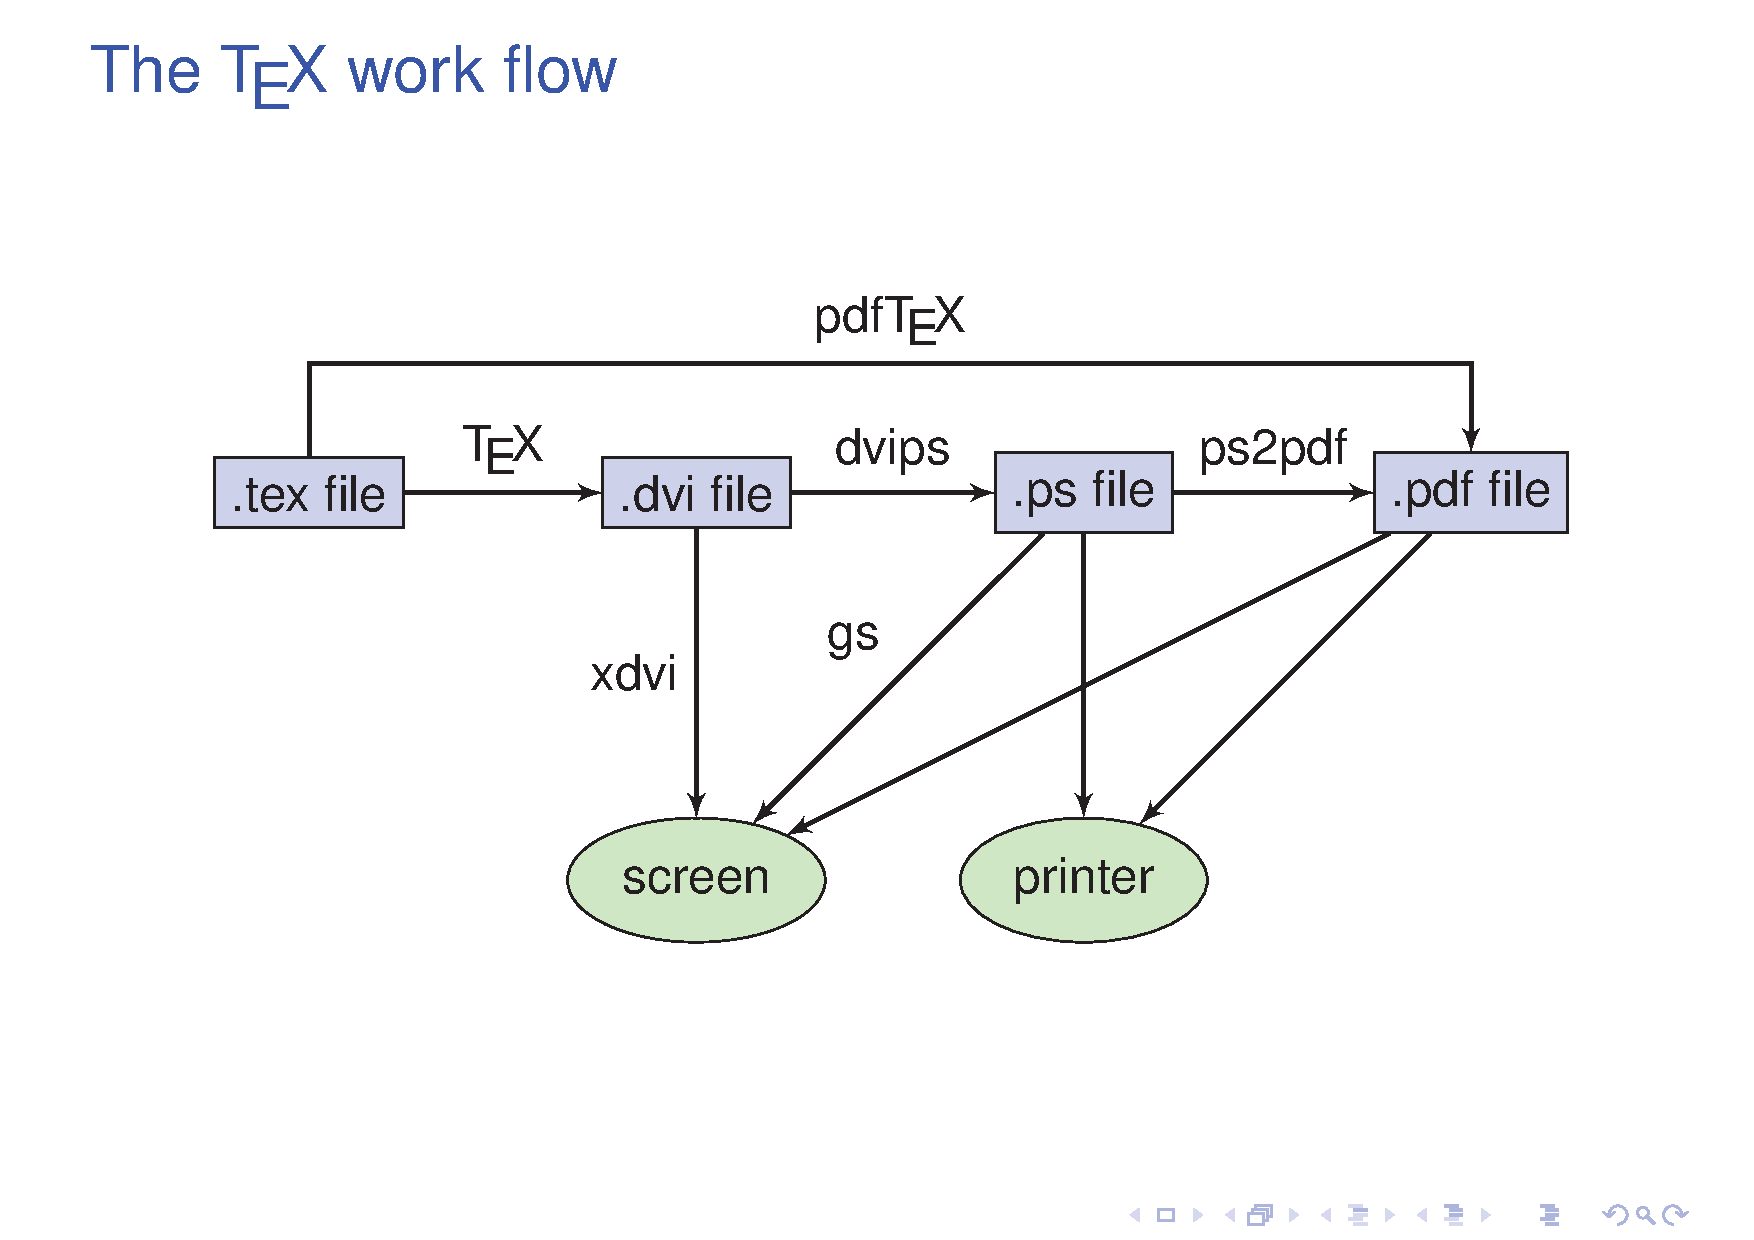
\includegraphics[width=\textwidth]{../graphs/tex-workflow.pdf}

Source: \href{http://media.texample.net/tikz/examples/PDF/tex-workflow.pdf}{http://media.texample.net/tikz/examples/PDF/tex-workflow.pdf}
\end{frame}
\begin{frame}[fragile,shrink = 5]
\frametitle{What a \LaTeX{} file looks like}
\label{sec-3_3}


\lstset{language=TeX}
\begin{lstlisting}
%% Part 1: Preamble
\documentclass{article} 

\usepackage[utf8]{inputenc}  
\usepackage[T1]{fontenc}
\usepackage[english]{babel}

%% Part 2: Body 
\begin{document}

\section{Heading} 

Hello world!

\begin{equation}
\overline{T} = \frac{\sum\limits^{k}_{i = 1} %
  T_{i}\cdot w_{i}}{\sum\limits^{k}_{i = 1}w_{i}}
\end{equation}

\end{document}
\end{lstlisting}
\end{frame}
\begin{frame}
\frametitle{The compiled 'Hello world'-example}
\label{sec-3_4}


\frame{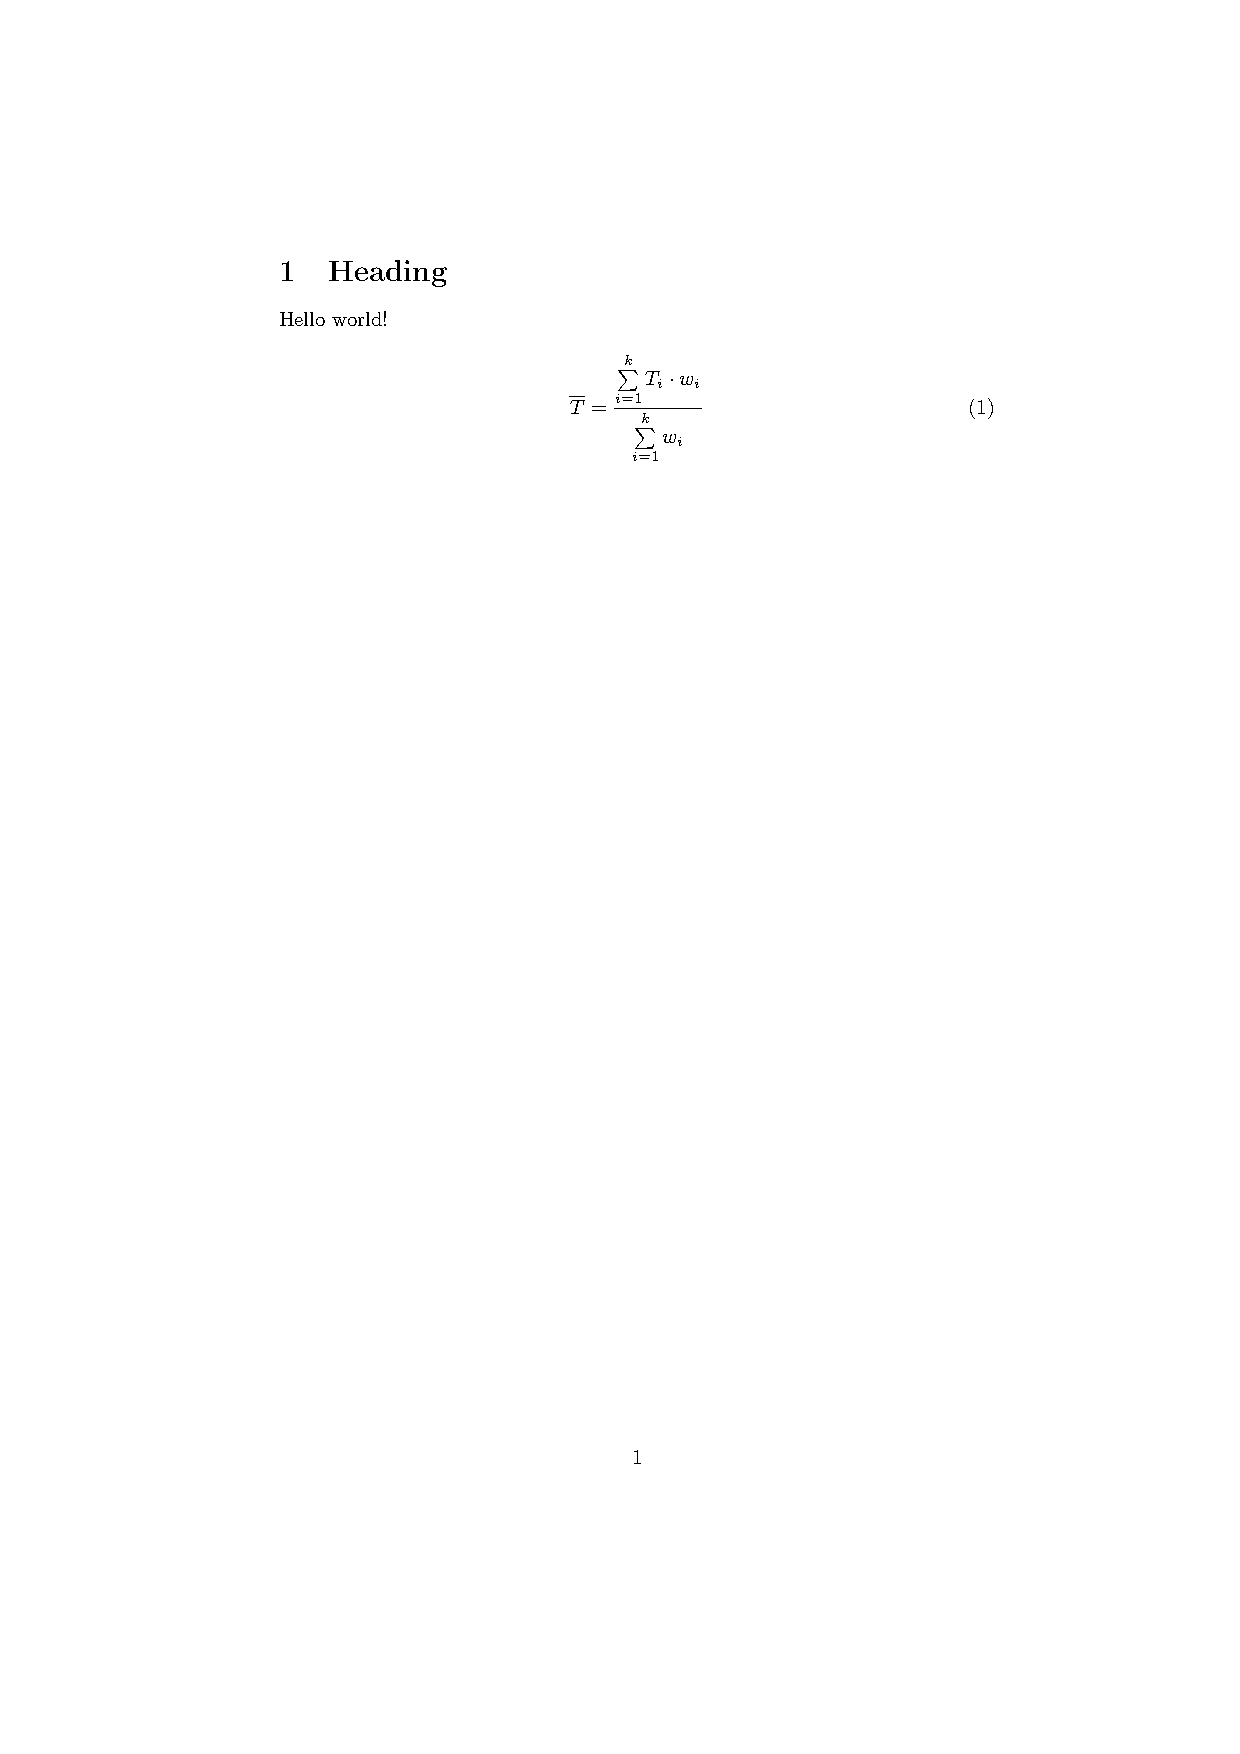
\includegraphics[clip, scale = 0.25]{hello_world.pdf}}
\end{frame}
\section{Sweave}
\label{sec-4}
\begin{frame}[fragile,shrink=10]
\frametitle{What a Sweave file looks like}
\label{sec-4_1}

\lstset{language=TeX}
\begin{lstlisting}
%% filename: src/tex/examp_sweave-01.Rnw
\documentclass[noae]{article}

\usepackage[utf8x]{inputenc}
\usepackage[T1]{fontenc}
\usepackage[english]{babel}
\usepackage[margin = 1in]{geometry}

\title{This is a tiny Sweave example}
\author{Bernd Weiss}

\begin{document}
\maketitle

I am using a built-in dataset which is called \texttt{USArrests} 
(Violent Crime Rates by US State).

<<echo = TRUE>>=
summary(USArrests)
@

The mean for "Murder arrests (per 100,000)" is \Sexpr{mean(USArrests$Murder)}.

\setkeys{Gin}{width=0.4\textwidth}

\begin{figure}[h!]
\begin{center}
<<echo = FALSE, fig = TRUE>>=
hist(USArrests$Murder)
@
\end{center}
\caption{Murder arrests (per 100,000)}
\end{figure}

\end{document}
\end{lstlisting}
\end{frame}
\begin{frame}[fragile]
\frametitle{Running Sweave}
\label{sec-4_2}


\lstset{language=R}
\begin{lstlisting}
setwd("E:/projects/software/reproducible_research/src/tex")
Sweave("examp_sweave-01.Rnw")
system("pdflatex -output-directory ../../slides examp_sweave-01.tex", 
       show.output.on.console = TRUE,
       minimized = FALSE)
\end{lstlisting}
\end{frame}
\begin{frame}
\frametitle{The compiled Sweave-example}
\label{sec-4_3}


\frame{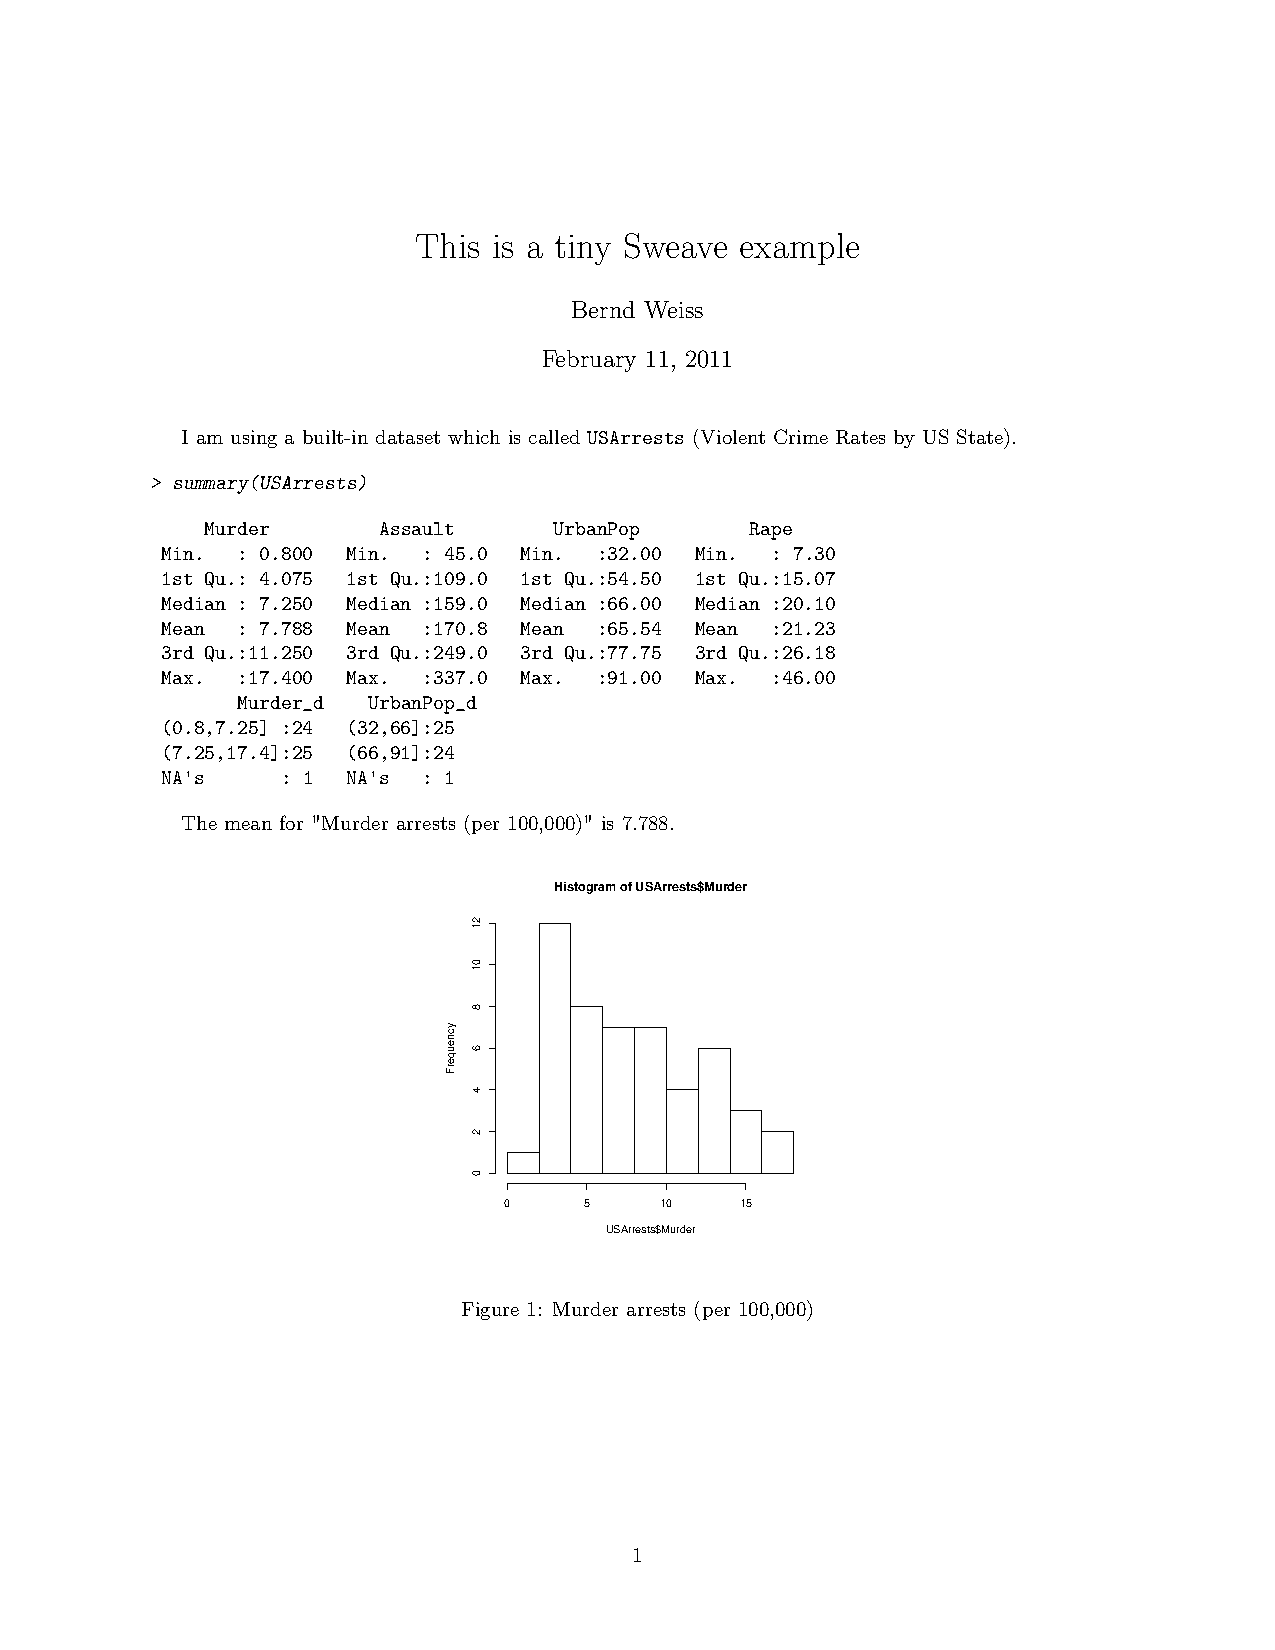
\includegraphics[clip, scale = 0.28]{examp_sweave-01.pdf}}
\end{frame}
\begin{frame}[fragile,shrink=10]
\frametitle{A second Sweave example}
\label{sec-4_4}

\lstset{language=TeX}
\begin{lstlisting}
%% filename: src/tex/examp_sweave-02.Rnw
\documentclass[noae]{article}

\usepackage[utf8x]{inputenc}
\usepackage[T1]{fontenc}
\usepackage[english]{babel}

\title{This is a tiny Sweave example}
\author{Bernd Weiss}

\begin{document}
\maketitle

How to create publication-ready table:

<<echo = FALSE, results = tex>>=
library(xtable)
USArrests$Murder_d <- cut(USArrests$Murder, 
                          quantile(USArrests$Murder, 
                          probs = seq(0, 1, 0.5)))
USArrests$UrbanPop_d <- cut(USArrests$UrbanPop, 
                            quantile(USArrests$UrbanPop, 
                            probs = seq(0, 1, 0.5)))
xtable(table(USArrests$Murder_d, USArrests$UrbanPop_d))
@


<<echo = FALSE, results = tex>>=

xtable(lm(Murder ~ UrbanPop, data = USArrests))
@

\end{document}
\end{lstlisting}
\end{frame}
\begin{frame}
\frametitle{The second compiled Sweave-example}
\label{sec-4_5}


\frame{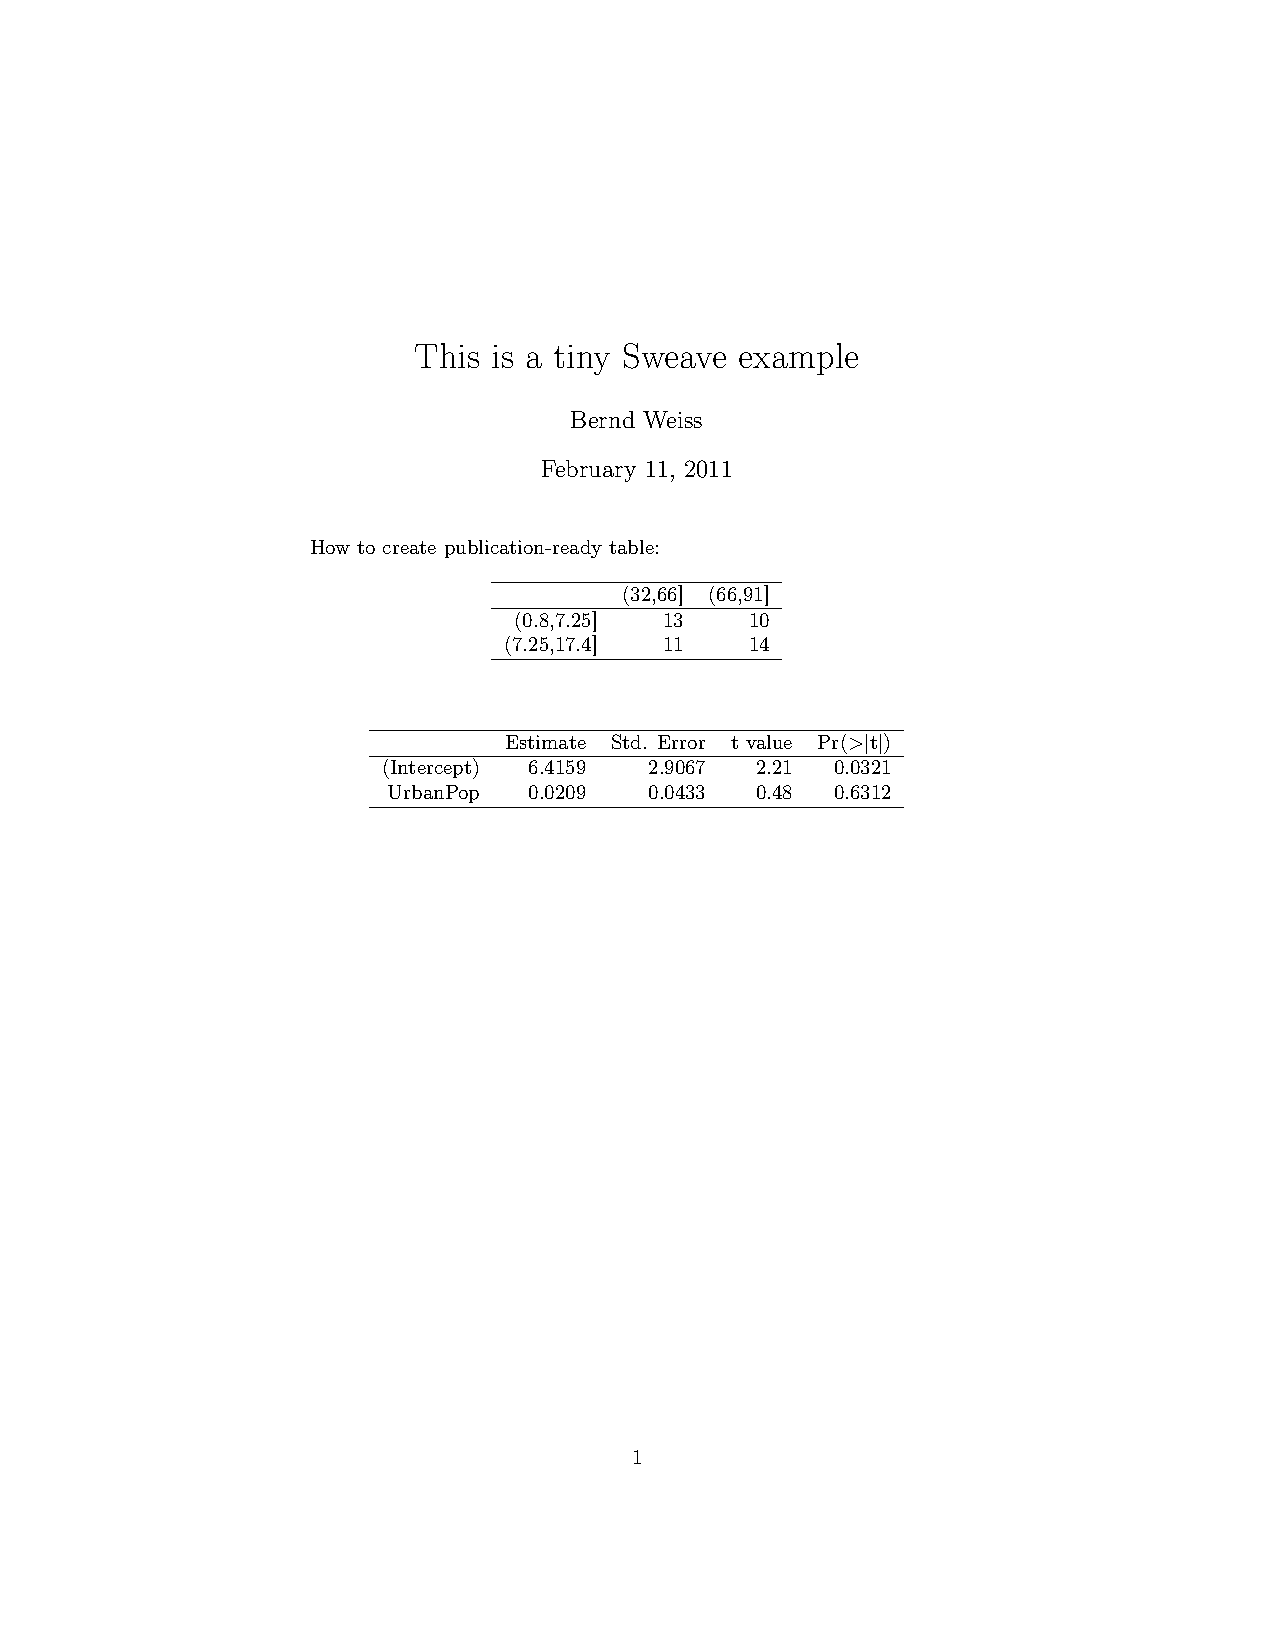
\includegraphics[clip, scale = 0.28]{examp_sweave-02.pdf}}
\end{frame}
\section{References and additional materials}
\label{sec-5}
\begin{frame}
\frametitle{(Some) R packages that generate \LaTeX{} code}
\label{sec-5_1}
\begin{itemize}

\item \href{http://cran.r-project.org/web/packages/Hmisc/index.html}{Hmisc: Harrell Miscellaneous}\\
\label{sec-5_1_1}%
\item \href{http://cran.r-project.org/web/packages/memisc/index.html}{memisc: Tools for Management of Survey Data, Graphics, Programming, Statistics, and Simulation}\\
\label{sec-5_1_2}%
\item \href{http://cran.r-project.org/web/packages/reporttools/}{reporttools: Generate \LaTeX{} tables of descriptive statistics}\\
\label{sec-5_1_3}%
\item \href{http://cran.r-project.org/web/packages/xtable/index.html}{xtable: Export tables to \LaTeX{} or HTML}\\
\label{sec-5_1_4}%
\item \ldots\\
\label{sec-5_1_5}%
\item For a general overview see \href{http://cran.r-project.org/web/views/ReproducibleResearch.html}{CRAN Task View: Reproducible Research}\\
\label{sec-5_1_6}%
\end{itemize} % ends low level
\end{frame}
\begin{frame}
\frametitle{R related materials}
\label{sec-5_2}
\begin{itemize}

\item \href{http://www.stat.uni-muenchen.de/~leisch/Sweave/}{Friedrich Leisch's The Sweave Homepage}\\
\label{sec-5_2_1}%
\item \href{http://www.stat.umn.edu/~charlie/Sweave/}{An Sweave Demo, Literate Programming in R, Reproducible Research }\\
\label{sec-5_2_2}%
\item Jeromy Anglim's talk about "\href{http://jeromyanglim.blogspot.com/2010/12/r-workflow-slides-from-talk-at.html}{R Workflow: Slides from a Talk at Melbourne R Users (1st Dec 2010)}" (Slides + Video)\\
\label{sec-5_2_3}%
\item Tal Galili: \href{http://www.r-statistics.com/2010/05/exporting-r-output-to-ms-word-with-r2wd-an-example-session/}{Exporting R output to MS-Word with R2wd (an example session)}\\
\label{sec-5_2_4}%
\item \href{http://cran.r-project.org/web/views/ReproducibleResearch.html}{CRAN Task View: Reproducible Research}\\
\label{sec-5_2_5}%
\item \href{http://book-by-sweave.wikidot.com/}{A Sweave Wiki}\\
\label{sec-5_2_6}%
\item \href{http://www.stat.auckland.ac.nz/~stat782/downloads/Sweave-customisation.pdf}{Customizing Sweave to Produce Better Looking \LaTeX{} Output}\\
\label{sec-5_2_7}%
\end{itemize} % ends low level
\end{frame}
\begin{frame}
\frametitle{Reproducible research related materials}
\label{sec-5_3}
\begin{itemize}

\item \href{http://bib.oxfordjournals.org/content/early/2011/01/28/bib.bbq084.abstract}{Hothorn/Leisch (2011): Case studies in reproducibility }\\
\label{sec-5_3_1}%
\item \href{http://reproducibleresearch.net/index.php/Main_Page}{ReproducibleResearch.net}\\
\label{sec-5_3_2}%
\item stackoverflow: \href{http://stackoverflow.com/questions/1429907/workflow-for-statistical-analysis-and-report-writing/}{Workflow for statistical analysis and report writing}\\
\label{sec-5_3_3}%
\item \href{http://www.bepress.com/bioconductor/paper2/}{Gentleman/Lang (2004): Statistical Analyses and Reproducible Research}\\
\label{sec-5_3_4}%
\end{itemize} % ends low level
\end{frame}

\end{document}